\documentclass{article}

\usepackage{amsmath}
\usepackage{minted}
\usepackage{graphicx}
\usepackage{caption}
\usepackage{subcaption}
\usepackage{mathrsfs}
\usepackage[toc,page]{appendix}

%Section style
\usepackage{etoolbox} %for configuration of sloppy
\usepackage{xcolor}


\definecolor{secnum}{RGB}{102,102,102}

\makeatletter
    \def\@seccntformat#1{\llap{\color{secnum}\csname the#1\endcsname\hskip 16pt}}
\makeatother
%end section style

\begin{document}

\section{I.2}

\subsection{I.2.1}

We are using the guassian function:
\begin{equation}
    f(x) = a * exp\left(-\frac{(x-b)^2}{2c^2}\right)
\end{equation}
Where:
\begin{align*}
    a &= \frac{1}{\sigma \sqrt{2\pi}}\\
    b &= \mu\\
    c &= \sigma 
\end{align*}
Giving us the full equation:
\begin{equation}
    f(x) = \frac{1}{\sigma \sqrt{2\pi}} * exp\left(-\frac{(x-\mu)^2}{2\sigma^2}\right)
\end{equation}


\begin{figure}[!ht]
    \centering
    \begin{subfigure}[b]{0.4\textwidth}
        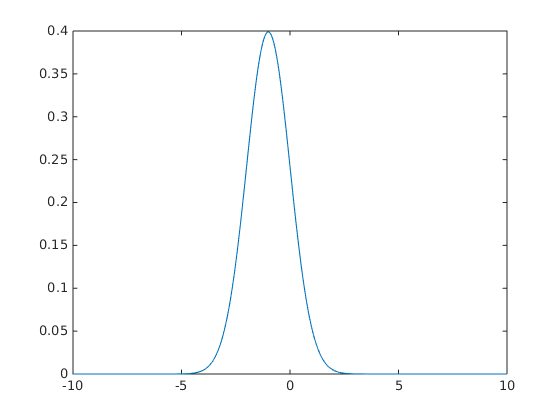
\includegraphics[width=\textwidth]{part1/I211.png}
        \caption{$(\mu, \sigma) = (-1,1)$}
    \end{subfigure}%
    \begin{subfigure}[b]{0.4\textwidth}
        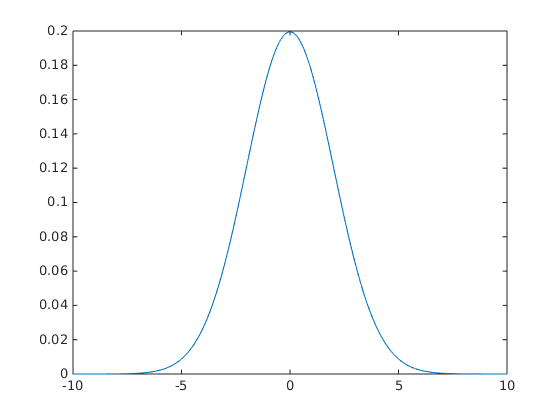
\includegraphics[width=\textwidth]{part1/I212.png}
        \caption{$(\mu, \sigma) = (0,2)$}
    \end{subfigure}
    \begin{subfigure}[b]{0.4\textwidth}
        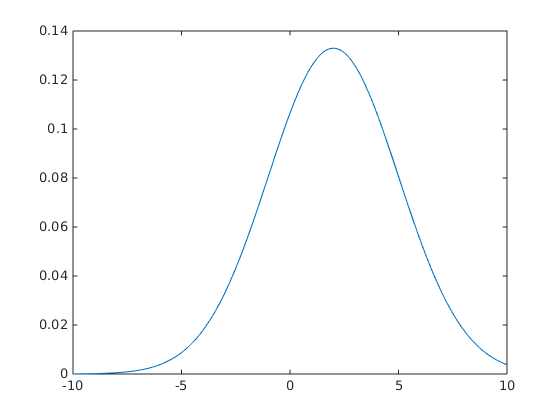
\includegraphics[width=\textwidth]{part1/I213.png}
        \caption{$(\mu, \sigma) = (2,3)$}
    \end{subfigure}
    \caption{Gaussian distribution with varying parameters}
    \label{fig:I1.1}
\end{figure}

Using matlab we implemented (2), giving us the figures \ref{fig:I1.1}

\subsection{I2.2}


We created two sets of normal distribution $\mathscr{N}(0,1)$, and extracted a sample with the distribution of $\mathscr{N}(y \| \mu, \sum)$ 
with mean:

\begin{equation}\label{eq:2.2mean}
    \mu = (1,2)^T
\end{equation} 
and covariance:

\begin{equation}\label{eq:2.2co}
    \sum = \left( \begin{array}{cc} 0.3 & 0.2 \\ 0.2 & 0.2 \end{array} \right)
\end{equation}


This gave us the plots seen on Figure \ref{fig:I2.2}

\begin{figure}[!ht]
    \centering
    \begin{subfigure}[b]{0.5\textwidth}
        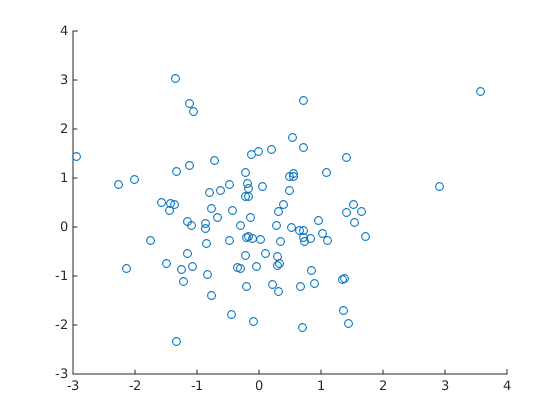
\includegraphics[width=\textwidth]{part1/I221.png}
        \caption{$\mathscr{N}(0,1)$ distribution}
    \end{subfigure}%
    \begin{subfigure}[b]{0.5\textwidth}
        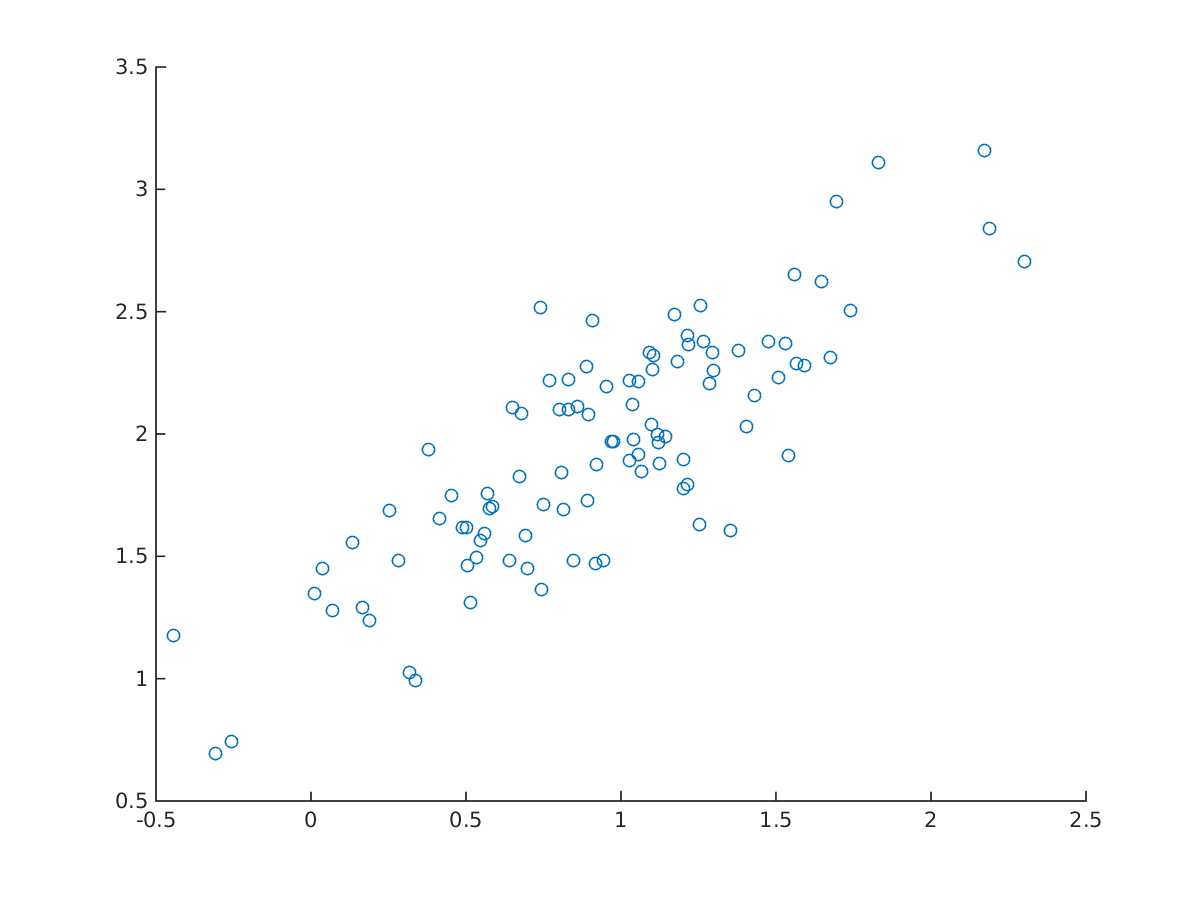
\includegraphics[width=\textwidth]{part1/I222.png}
        \caption{Sample distribution with (\ref{eq:2.2mean}) and (\ref{eq:2.2co})}
    \end{subfigure}
    \caption{Gaussian distribution with varying parameters}
    \label{fig:I2.2}
\end{figure}

\subsection{I2.3}


We calculated the mean of the dataset and plotted it ontop of the sampled
data together with the "actual" mean (1,2) as seen in \ref{fig:I3.1}

\begin{figure}[!ht]
    \centering
    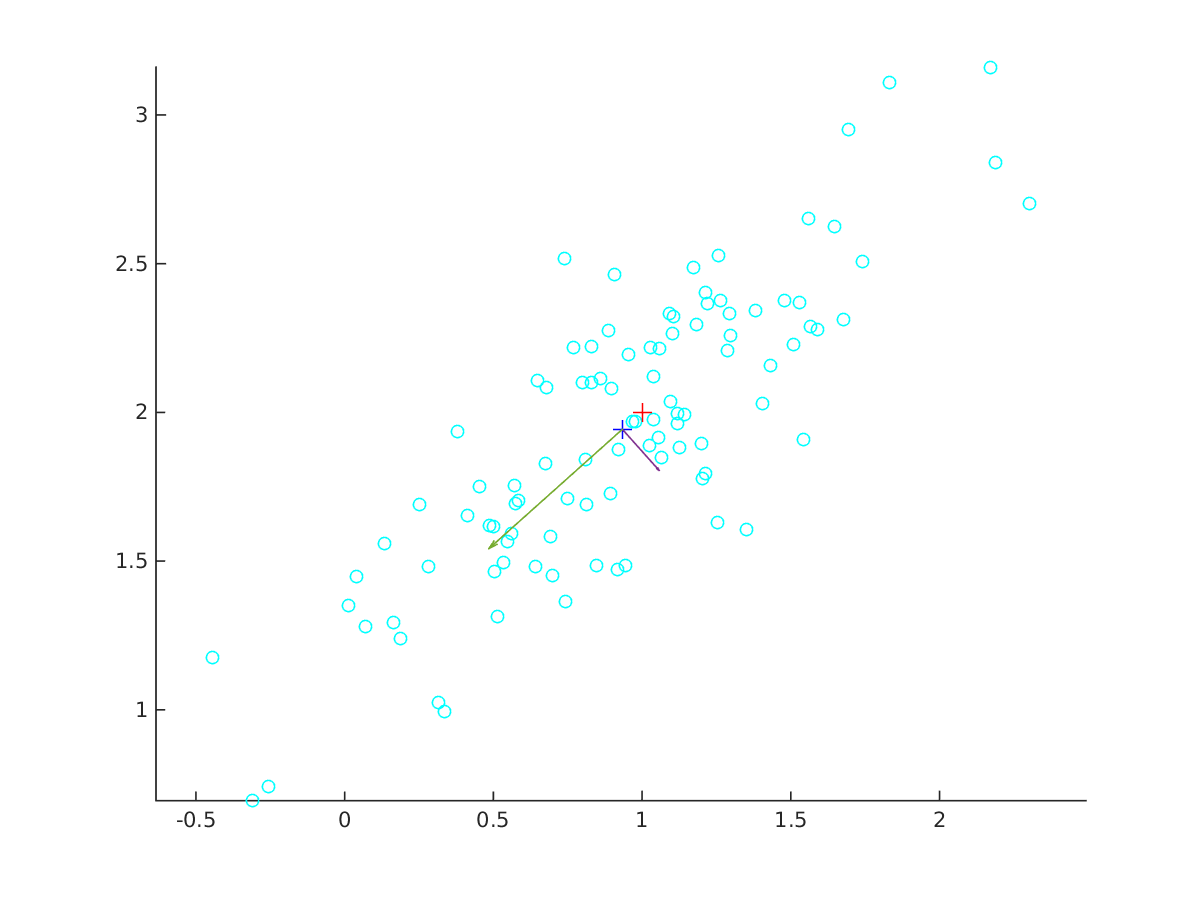
\includegraphics[width=\textwidth]{part1/I231.png}
    \caption{The dataset with the sample mean plotted as a blue '+' and
    distribution mean as a red '+'. The two eigenvectors are also plotted.}
    \label{fig:I3.1}
\end{figure}

The two points deviate because the sample is drawn from a random
distribution which does not necessarily give a sample balanced around the
mean of the distribution. As the amount of datapoints in the sample
increase, the mean should approach the distribution mean.


\subsection{I2.4}

The eigenvectors are plotted in figure \ref{fig:I3.1} and describe in which
directions the sample spreads and the eigenvalues describe how heavily it
spreads in the respective direction.

\begin{figure}[!ht]
    \centering
    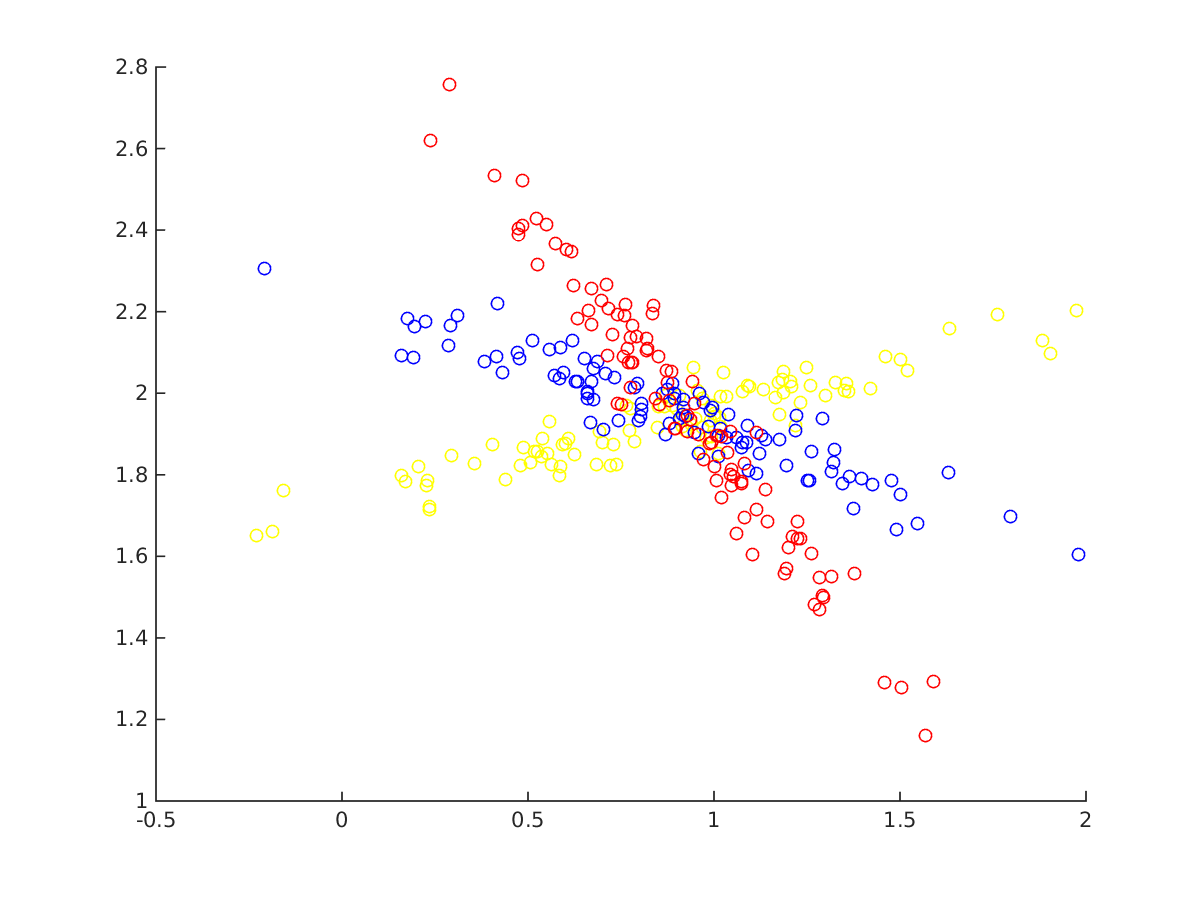
\includegraphics[width=\textwidth]{part1/I241.png}
    \caption{Three different rotations of the sample. The yellow one is
    rotated 30 degrees, the blue one 60 and the red 90.}
    \label{fig:I4.1}
\end{figure}

\begin{figure}[!ht]
    \centering
    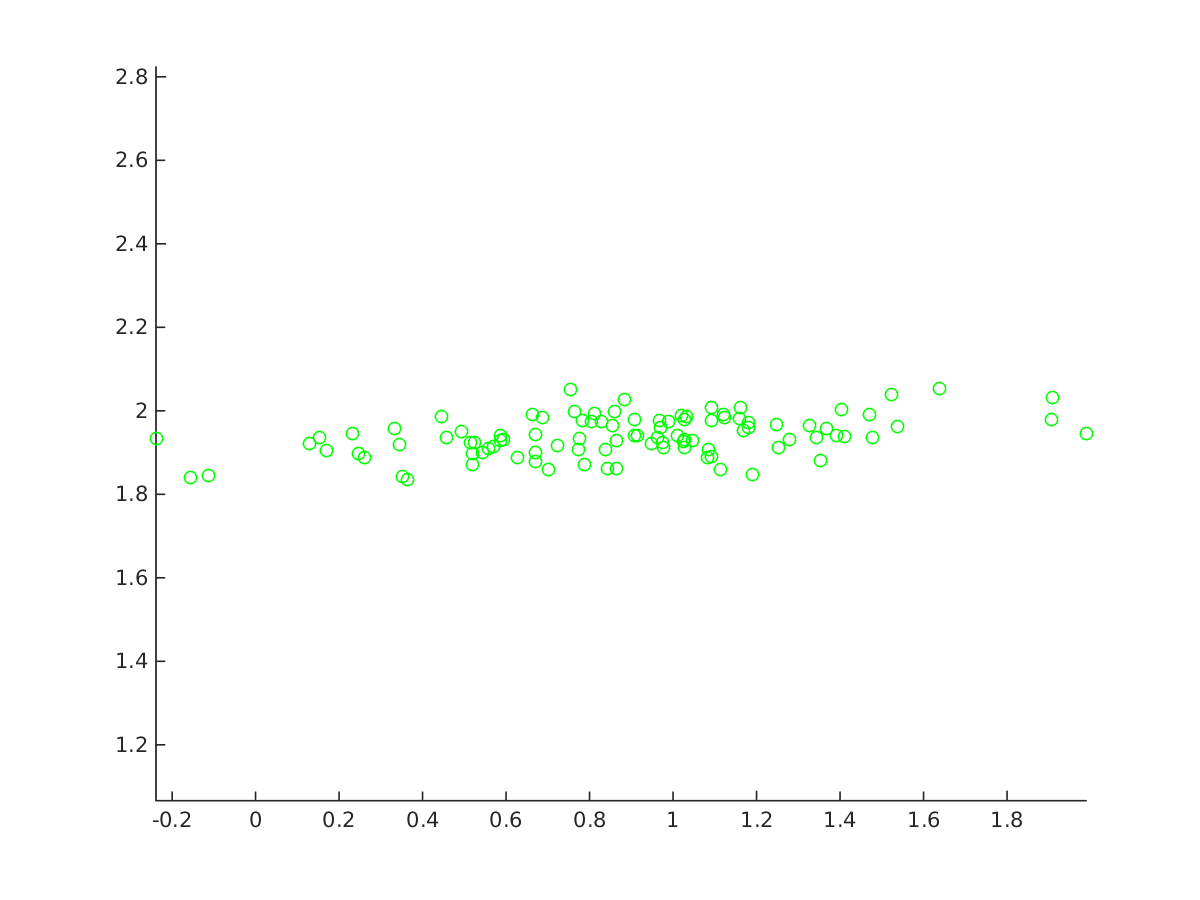
\includegraphics[width=\textwidth]{part1/I242.png}
    \caption{The sample rotated 40 degrees.}
    \label{fig:I4.2}
\end{figure}

The rotated samples are plotted in figure \ref{fig:I4.1}. As seen in
figure \ref{fig:I4.2} is looks likes a rotation of 40 degrees will just
about tilt it to lie parallel to the x-axis.




\section{I.3}


\subsection{I.3.1}

We ran the code and got the following results from $k = \{1,3,5\}$, using the training set for training and testing.\\ 

Hit ratio with 1 was 100.0\%. With 100.0 tries 100.0 hits and 0.0 misses\\
Hit ratio with 3 was 85.0\%. With 100.0 tries 85.0 hits and 15.0 misses\\
Hit ratio with 5 was 78.0\%. With 100.0 tries 78.0 hits and 22.0 misses
The best ratio was: 100.0 with a k value of 1


We ran the code and got the following results from $k = \{1,3,5\}$, using the training set for training and test set for testing.\\ 

Hit ratio with 1 was 81.5789473684\%. With 38.0 tries 31.0 hits and 7.0 misses\\
Hit ratio with 3 was 68.4210526316\%. With 38.0 tries 26.0 hits and 12.0 misses\\
Hit ratio with 5 was 60.5263157895\%. With 38.0 tries 23.0 hits and 15.0 misses\\
In both cases k = 1 is the best classifier. On the training data, it's
obviously perfect. \\\\

\subsection{I.3.2}

The cross-validation was done by splitting the test collection into
5 equal sizes, and running the code 5 times with one fifth of the full
collection as the test data and the rest as the training.\\\\ The code
was run as cross-validation with k-values ranging from 1 to 25 and the
data was not normalized. We chose to include the even numbers.\\\\
Average result:\\ 
Hit ratio with 1 was   78.0\%. With 20 tries 15.6 hits and 4.4 misses\\
Hit ratio with 2 was   79.0\%. With 20 tries 15.8 hits and 4.2 misses\\
Hit ratio with 3 was   76.0\%. With 20 tries 15.2 hits and 4.8 misses\\
Hit ratio with 4 was   75.0\%. With 20 tries 15.0 hits and 5.0 misses\\
Hit ratio with 5 was   74.0\%. With 20 tries 14.8 hits and 5.2 misses\\
Hit ratio with 6 was   74.0\%. With 20 tries 14.8 hits and 5.2 misses\\
Hit ratio with 7 was   74.0\%. With 20 tries 14.8 hits and 5.2 misses\\
Hit ratio with 8 was   78.0\%. With 20 tries 15.6 hits and 4.4 misses\\
Hit ratio with 9 was   77.0\%. With 20 tries 15.4 hits and 4.6 misses\\
Hit ratio with 10 was  78.0\%. With 20 tries 15.6 hits and 4.4 misses\\
Hit ratio with 11 was  78.0\%. With 20 tries 15.6 hits and 4.4 misses\\
Hit ratio with 12 was  77.0\%. With 20 tries 15.4 hits and 4.6 misses\\
Hit ratio with 13 was  75.0\%. With 20 tries 15.0 hits and 5.0 misses\\
Hit ratio with 14 was  76.0\%. With 20 tries 15.2 hits and 4.8 misses\\
Hit ratio with 15 was  78.0\%. With 20 tries 15.6 hits and 4.4 misses\\
Hit ratio with 16 was  77.0\%. With 20 tries 15.4 hits and 4.6 misses\\
Hit ratio with 17 was  76.0\%. With 20 tries 15.2 hits and 4.8 misses\\
Hit ratio with 18 was  76.0\%. With 20 tries 15.2 hits and 4.8 misses\\
Hit ratio with 19 was  75.0\%. With 20 tries 15.0 hits and 5.0 misses\\
Hit ratio with 20 was  76.0\%. With 20 tries 15.2 hits and 4.8 misses\\
Hit ratio with 21 was  73.0\%. With 20 tries 14.6 hits and 5.4 misses\\
Hit ratio with 22 was  75.0\%. With 20 tries 15.0 hits and 5.0 misses\\
Hit ratio with 23 was  75.0\%. With 20 tries 15.0 hits and 5.0 misses\\
Hit ratio with 24 was  71.0\%. With 20 tries 14.2 hits and 5.8 misses\\
Hit ratio with 25 was  73.0\%. With 20 tries 14.6 hits and 5.4 misses\\
The best ratio was: 79.0 with a k value of 2\\\\
Without normalizing the data, the k-value with the best result between the 5 runs was the one with a k of 2, with 1, 10 and 11 being secondbest.\\
k = 2 had an average miss rate of 4.2.

\subsection{I.3.3}

Type 0 has a mean of (4.93529411765, 0.335). An std of (0.298902259198, 0.0353345356806).\\
Type 1 has a mean of (5.69642857143, 0.2675). An std of (0.441977813646, 0.0295954871077).\\
Type 2 has a mean of (6.53421052632, 0.297105263158). An std of (0.614849710259, 0.0307714747211).\\
Overall mean is (5.756000000000003, 0.3017000000000001) and overall std is (0.82997831296968227, 0.041738591255575455)\\\\
Average result: \\
Hit ratio with 1 was   was 86.0\%. With 20 tries 17.2 hits and 2.8 misses\\
Hit ratio with 2 was   was 84.0\%. With 20 tries 16.8 hits and 3.2 misses\\
Hit ratio with 3 was   was 83.0\%. With 20 tries 16.6 hits and 3.4 misses\\
Hit ratio with 4 was   was 76.0\%. With 20 tries 15.2 hits and 4.8 misses\\
Hit ratio with 5 was   was 78.0\%. With 20 tries 15.6 hits and 4.4 misses\\
Hit ratio with 6 was   was 80.0\%. With 20 tries 16.0 hits and 4.0 misses\\
Hit ratio with 7 was   was 79.0\%. With 20 tries 15.8 hits and 4.2 misses\\
Hit ratio with 8 was   was 81.0\%. With 20 tries 16.2 hits and 3.8 misses\\
Hit ratio with 9 was   was 83.0\%. With 20 tries 16.6 hits and 3.4 misses\\
Hit ratio with 10 was  was 81.0\%. With 20 tries 16.2 hits and 3.8 misses\\
Hit ratio with 11 was  was 80.0\%. With 20 tries 16.0 hits and 4.0 misses\\
Hit ratio with 12 was  was 83.0\%. With 20 tries 16.6 hits and 3.4 misses\\
Hit ratio with 13 was  was 80.0\%. With 20 tries 16.0 hits and 4.0 misses\\
Hit ratio with 14 was  was 77.0\%. With 20 tries 15.4 hits and 4.6 misses\\
Hit ratio with 15 was  was 77.0\%. With 20 tries 15.4 hits and 4.6 misses\\
Hit ratio with 16 was  was 77.0\%. With 20 tries 15.4 hits and 4.6 misses\\
Hit ratio with 17 was  was 78.0\%. With 20 tries 15.6 hits and 4.4 misses\\
Hit ratio with 18 was  was 78.0\%. With 20 tries 15.6 hits and 4.4 misses\\
Hit ratio with 19 was  was 77.0\%. With 20 tries 15.4 hits and 4.6 misses\\
Hit ratio with 20 was  was 73.0\%. With 20 tries 14.6 hits and 5.4 misses\\
Hit ratio with 21 was  was 74.0\%. With 20 tries 14.8 hits and 5.2 misses\\
Hit ratio with 22 was  was 73.0\%. With 20 tries 14.6 hits and 5.4 misses\\
Hit ratio with 23 was  was 73.0\%. With 20 tries 14.6 hits and 5.4 misses\\
Hit ratio with 24 was  was 74.0\%. With 20 tries 14.8 hits and 5.2 misses\\
Hit ratio with 25 was  was 72.0\%. With 20 tries 14.4 hits and 5.6 misses\\
The best ratio was: 86.0 with a k value of 1\\\\
After the transformation the distribution of the data on both axis is $\mathscr{N}(0,1)$. Our best k from the 
cross validation before normalization was 2 with a hit percent of 79\%, this was improved to 84\% by the normalization. 
A k of 1 is however better with a hit percentage of 86\%, giving us an average of 2.8 misses on 20 tries.\\
We presume this is because the normalization made the delta length on the y axis more significant, as they previously was smaller by a factor of 10,
and through this the difference on that axis had very little impact on the choice.

\end{document}
